% P05 diagnostic figure best_epoch_distribution|held_evaluation|guard_selection_fit; allowlisted public aggregate points.
% Each point is an aggregate mean or bin over repeated contexts, not an independent sample.
% data_sha256=7f60e425b5fe235c362c21442c3237e1521aad33df8bebdebfd5854e0cfadd4b
\documentclass[tikz,border=5pt]{standalone}
\ifdefined\pdfinfoomitdate\pdfinfoomitdate=1\fi
\ifdefined\pdfsuppressptexinfo\pdfsuppressptexinfo=-1\fi
\ifdefined\pdftrailerid\pdftrailerid{}\fi
\usepackage{pgfplots}
\usepgfplotslibrary{groupplots}
\pgfplotsset{compat=1.18}
\definecolor{p05Blue}{HTML}{0072B2}
\definecolor{p05Orange}{HTML}{E69F00}
\definecolor{p05Green}{HTML}{009E73}
\definecolor{p05Purple}{HTML}{CC79A7}
\definecolor{p05Red}{HTML}{D55E00}
\definecolor{p05Sky}{HTML}{56B4E9}
\begin{document}
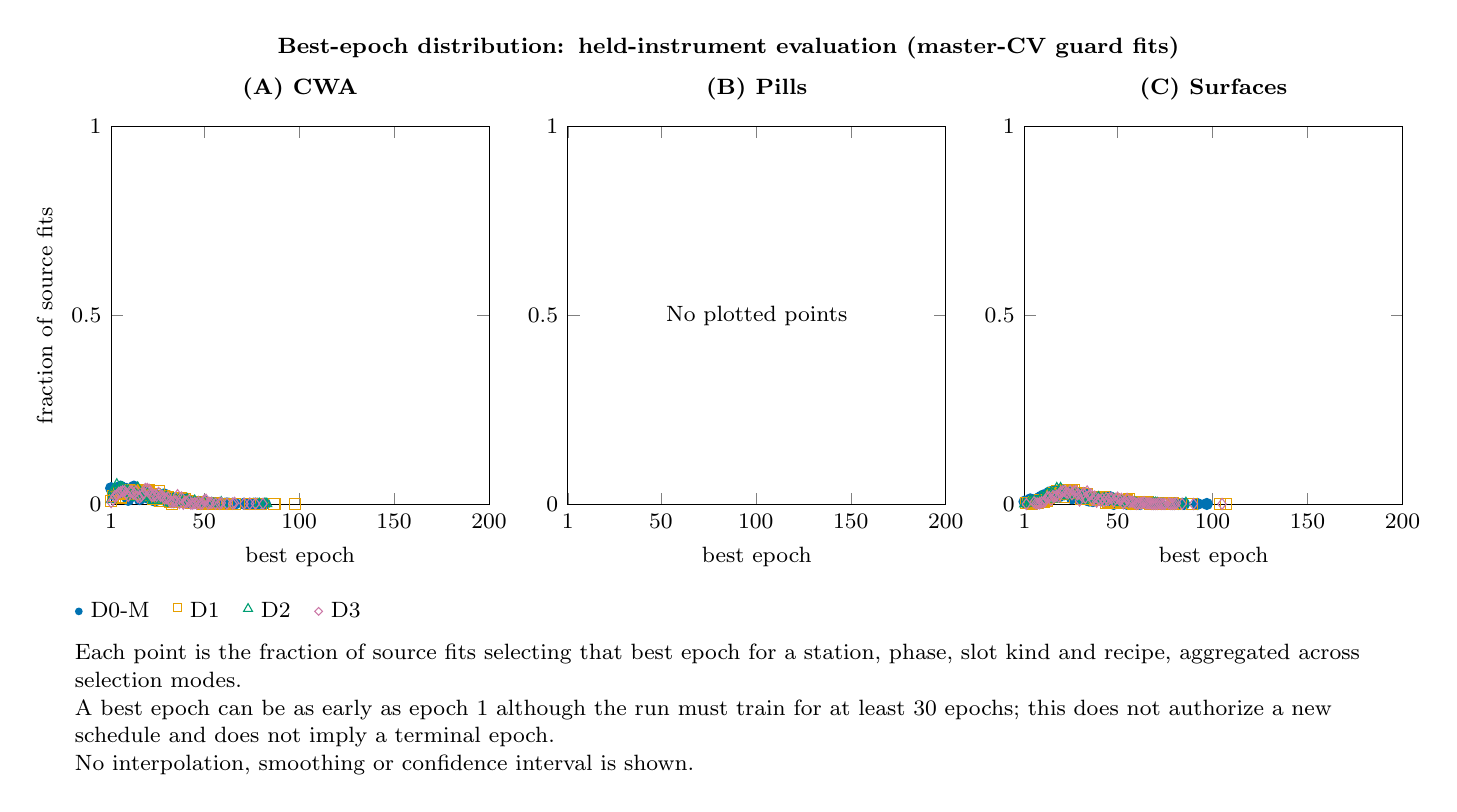
\begin{tikzpicture}
\begin{groupplot}[
  group style={group size=3 by 1, horizontal sep=1.0cm, vertical sep=1.8cm},
  width=4.8cm, height=4.8cm, scale only axis,
  xmin=1, xmax=200, ymin=0, ymax=1,
  xtick={1,50,100,150,200}, ytick={0,0.5,1},
  tick label style={font=\fontsize{8}{10}\selectfont, color=black},
  label style={font=\fontsize{8}{10}\selectfont, color=black},
  title style={font=\fontsize{8}{10}\selectfont\bfseries, color=black},
]
\nextgroupplot[title={(A) CWA}, xlabel={best epoch}, ylabel={fraction of source fits}]
\addplot[only marks, mark=*, mark size=2.0pt, color=p05Blue, mark options={fill=p05Blue, draw=p05Blue}] coordinates {(1,0.043209876543209874) (2,0.026748971193415638) (3,0.037037037037037035) (4,0.041152263374485597) (5,0.028806584362139918) (6,0.047325102880658436) (7,0.03292181069958848) (8,0.03292181069958848) (9,0.041152263374485597) (10,0.012345679012345678) (11,0.028806584362139918) (12,0.03292181069958848) (13,0.047325102880658436) (14,0.026748971193415638) (15,0.026748971193415638) (16,0.014403292181069959) (17,0.022633744855967079) (18,0.020576131687242798) (19,0.03292181069958848) (20,0.024691358024691357) (21,0.01646090534979424) (22,0.018518518518518517) (23,0.012345679012345678) (24,0.010288065843621399) (25,0.024691358024691357) (26,0.020576131687242798) (27,0.020576131687242798) (28,0.022633744855967079) (29,0.026748971193415638) (30,0.010288065843621399) (31,0.00823045267489712) (32,0.020576131687242798) (33,0.00823045267489712) (34,0.0061728395061728392) (35,0.012345679012345678) (36,0.014403292181069959) (37,0.0061728395061728392) (38,0.00823045267489712) (39,0.014403292181069959) (40,0.014403292181069959) (41,0.00411522633744856) (42,0.00823045267489712) (43,0.00411522633744856) (44,0.0061728395061728392) (45,0.00411522633744856) (47,0.0061728395061728392) (48,0.0061728395061728392) (49,0.00411522633744856) (50,0.00823045267489712) (52,0.00205761316872428) (54,0.00205761316872428) (58,0.00411522633744856) (61,0.00205761316872428) (62,0.00205761316872428) (63,0.00205761316872428) (65,0.00205761316872428) (66,0.00205761316872428) (71,0.00205761316872428) (74,0.00205761316872428) (76,0.00205761316872428) (77,0.00205761316872428) (78,0.00205761316872428) (82,0.00205761316872428)};
\addplot[only marks, mark=square, mark size=2.0pt, color=p05Orange, mark options={fill=none, draw=p05Orange}] coordinates {(1,0.010288065843621399) (2,0.022633744855967079) (3,0.020576131687242798) (4,0.030864197530864196) (5,0.030864197530864196) (6,0.018518518518518517) (7,0.026748971193415638) (8,0.030864197530864196) (9,0.039094650205761319) (10,0.03292181069958848) (11,0.037037037037037035) (12,0.028806584362139918) (13,0.034979423868312758) (14,0.028806584362139918) (15,0.030864197530864196) (16,0.028806584362139918) (17,0.037037037037037035) (18,0.03292181069958848) (19,0.039094650205761319) (20,0.03292181069958848) (21,0.037037037037037035) (22,0.024691358024691357) (23,0.014403292181069959) (24,0.028806584362139918) (25,0.014403292181069959) (26,0.034979423868312758) (27,0.010288065843621399) (28,0.020576131687242798) (29,0.022633744855967079) (30,0.018518518518518517) (31,0.018518518518518517) (32,0.0061728395061728392) (33,0.00205761316872428) (34,0.0061728395061728392) (35,0.010288065843621399) (36,0.010288065843621399) (37,0.0061728395061728392) (38,0.01646090534979424) (39,0.014403292181069959) (40,0.014403292181069959) (41,0.00823045267489712) (42,0.00823045267489712) (43,0.00411522633744856) (44,0.00411522633744856) (45,0.00411522633744856) (46,0.00411522633744856) (47,0.0061728395061728392) (48,0.00411522633744856) (49,0.00205761316872428) (52,0.00205761316872428) (53,0.00411522633744856) (55,0.00411522633744856) (57,0.00205761316872428) (58,0.00205761316872428) (61,0.00205761316872428) (62,0.00205761316872428) (66,0.00205761316872428) (74,0.00205761316872428) (80,0.00205761316872428) (87,0.00205761316872428) (98,0.00205761316872428)};
\addplot[only marks, mark=triangle, mark size=2.0pt, color=p05Green, mark options={fill=none, draw=p05Green}] coordinates {(1,0.012345679012345678) (2,0.037037037037037035) (3,0.043209876543209874) (4,0.053497942386831275) (5,0.039094650205761319) (6,0.045267489711934158) (7,0.045267489711934158) (8,0.030864197530864196) (9,0.037037037037037035) (10,0.037037037037037035) (11,0.028806584362139918) (12,0.018518518518518517) (13,0.03292181069958848) (14,0.026748971193415638) (15,0.045267489711934158) (16,0.024691358024691357) (17,0.024691358024691357) (18,0.01646090534979424) (19,0.020576131687242798) (20,0.030864197530864196) (21,0.024691358024691357) (22,0.022633744855967079) (23,0.010288065843621399) (24,0.020576131687242798) (25,0.010288065843621399) (26,0.018518518518518517) (27,0.014403292181069959) (28,0.024691358024691357) (29,0.014403292181069959) (30,0.020576131687242798) (31,0.01646090534979424) (32,0.00411522633744856) (33,0.00411522633744856) (34,0.01646090534979424) (35,0.00411522633744856) (36,0.00823045267489712) (37,0.014403292181069959) (38,0.0061728395061728392) (39,0.012345679012345678) (41,0.014403292181069959) (42,0.0061728395061728392) (43,0.0061728395061728392) (44,0.00205761316872428) (45,0.010288065843621399) (46,0.00205761316872428) (47,0.0061728395061728392) (48,0.00411522633744856) (49,0.00205761316872428) (50,0.0061728395061728392) (54,0.00411522633744856) (55,0.00205761316872428) (56,0.00205761316872428) (59,0.0061728395061728392) (62,0.00205761316872428) (79,0.00205761316872428) (82,0.00205761316872428) (83,0.00205761316872428)};
\addplot[only marks, mark=diamond, mark size=2.0pt, color=p05Purple, mark options={fill=none, draw=p05Purple}] coordinates {(1,0.0061728395061728392) (2,0.012345679012345678) (3,0.022633744855967079) (4,0.024691358024691357) (5,0.030864197530864196) (6,0.03292181069958848) (7,0.034979423868312758) (8,0.034979423868312758) (9,0.028806584362139918) (10,0.022633744855967079) (11,0.034979423868312758) (12,0.034979423868312758) (13,0.028806584362139918) (14,0.034979423868312758) (15,0.020576131687242798) (16,0.018518518518518517) (17,0.022633744855967079) (18,0.028806584362139918) (19,0.041152263374485597) (20,0.041152263374485597) (21,0.039094650205761319) (22,0.024691358024691357) (23,0.022633744855967079) (24,0.024691358024691357) (25,0.022633744855967079) (26,0.030864197530864196) (27,0.022633744855967079) (28,0.022633744855967079) (29,0.01646090534979424) (30,0.01646090534979424) (31,0.018518518518518517) (32,0.00823045267489712) (33,0.0061728395061728392) (34,0.00823045267489712) (35,0.00823045267489712) (36,0.024691358024691357) (37,0.00411522633744856) (38,0.018518518518518517) (39,0.00205761316872428) (40,0.0061728395061728392) (41,0.0061728395061728392) (42,0.010288065843621399) (43,0.00205761316872428) (44,0.00205761316872428) (45,0.00411522633744856) (46,0.00205761316872428) (47,0.0061728395061728392) (48,0.00205761316872428) (49,0.00205761316872428) (50,0.010288065843621399) (51,0.012345679012345678) (52,0.00205761316872428) (53,0.00411522633744856) (54,0.00411522633744856) (56,0.00205761316872428) (58,0.00205761316872428) (59,0.00411522633744856) (62,0.00205761316872428) (65,0.00205761316872428) (66,0.00411522633744856) (71,0.00205761316872428) (74,0.00205761316872428) (77,0.00205761316872428) (81,0.00205761316872428)};
\nextgroupplot[title={(B) Pills}, xlabel={best epoch}]
\node[font=\fontsize{8}{10}\selectfont,align=center] at (axis cs:100.5,0.5) {No plotted points};
\nextgroupplot[title={(C) Surfaces}, xlabel={best epoch}]
\addplot[only marks, mark=*, mark size=2.0pt, color=p05Blue, mark options={fill=p05Blue, draw=p05Blue}] coordinates {(1,0.0075075075075075074) (2,0.003003003003003003) (3,0.0045045045045045045) (4,0.013513513513513514) (5,0.012012012012012012) (6,0.0075075075075075074) (7,0.010510510510510511) (8,0.013513513513513514) (9,0.018018018018018018) (10,0.021021021021021023) (11,0.024024024024024024) (12,0.018018018018018018) (13,0.021021021021021023) (14,0.031531531531531529) (15,0.031531531531531529) (16,0.034534534534534533) (17,0.022522522522522521) (18,0.028528528528528527) (19,0.021021021021021023) (20,0.03903903903903904) (21,0.027027027027027029) (22,0.027027027027027029) (23,0.034534534534534533) (24,0.028528528528528527) (25,0.027027027027027029) (26,0.016516516516516516) (27,0.024024024024024024) (28,0.021021021021021023) (29,0.016516516516516516) (30,0.03003003003003003) (31,0.022522522522522521) (32,0.024024024024024024) (33,0.028528528528528527) (34,0.012012012012012012) (35,0.010510510510510511) (36,0.01951951951951952) (37,0.0090090090090090089) (38,0.013513513513513514) (39,0.015015015015015015) (40,0.01951951951951952) (41,0.015015015015015015) (42,0.010510510510510511) (43,0.016516516516516516) (44,0.013513513513513514) (45,0.015015015015015015) (46,0.01951951951951952) (47,0.006006006006006006) (48,0.0015015015015015015) (49,0.010510510510510511) (50,0.010510510510510511) (51,0.0090090090090090089) (52,0.0045045045045045045) (53,0.0075075075075075074) (54,0.0075075075075075074) (55,0.0015015015015015015) (56,0.0075075075075075074) (57,0.0015015015015015015) (60,0.003003003003003003) (61,0.0015015015015015015) (62,0.0015015015015015015) (63,0.0045045045045045045) (65,0.0045045045045045045) (69,0.0015015015015015015) (70,0.003003003003003003) (71,0.0045045045045045045) (79,0.0015015015015015015) (80,0.0015015015015015015) (82,0.0015015015015015015) (85,0.0015015015015015015) (92,0.0015015015015015015) (97,0.0015015015015015015)};
\addplot[only marks, mark=square, mark size=2.0pt, color=p05Orange, mark options={fill=none, draw=p05Orange}] coordinates {(2,0.003003003003003003) (3,0.003003003003003003) (4,0.003003003003003003) (5,0.0015015015015015015) (6,0.006006006006006006) (7,0.0075075075075075074) (8,0.0045045045045045045) (9,0.012012012012012012) (10,0.0075075075075075074) (11,0.006006006006006006) (12,0.012012012012012012) (13,0.010510510510510511) (14,0.018018018018018018) (15,0.021021021021021023) (16,0.03003003003003003) (17,0.021021021021021023) (18,0.036036036036036036) (19,0.028528528528528527) (20,0.027027027027027029) (21,0.03003003003003003) (22,0.021021021021021023) (23,0.03903903903903904) (24,0.033033033033033031) (25,0.028528528528528527) (26,0.034534534534534533) (27,0.037537537537537538) (28,0.028528528528528527) (29,0.027027027027027029) (30,0.03003003003003003) (31,0.015015015015015015) (32,0.027027027027027029) (33,0.027027027027027029) (34,0.027027027027027029) (35,0.01951951951951952) (36,0.016516516516516516) (37,0.013513513513513514) (38,0.012012012012012012) (39,0.016516516516516516) (40,0.01951951951951952) (41,0.016516516516516516) (42,0.015015015015015015) (43,0.01951951951951952) (44,0.0045045045045045045) (45,0.006006006006006006) (46,0.010510510510510511) (47,0.015015015015015015) (48,0.015015015015015015) (49,0.0090090090090090089) (50,0.0045045045045045045) (51,0.010510510510510511) (52,0.006006006006006006) (53,0.0090090090090090089) (54,0.0090090090090090089) (55,0.010510510510510511) (56,0.015015015015015015) (57,0.0045045045045045045) (58,0.0015015015015015015) (59,0.003003003003003003) (60,0.0045045045045045045) (61,0.006006006006006006) (63,0.006006006006006006) (64,0.003003003003003003) (65,0.003003003003003003) (66,0.006006006006006006) (67,0.0015015015015015015) (68,0.0015015015015015015) (69,0.003003003003003003) (70,0.0015015015015015015) (71,0.0015015015015015015) (73,0.0015015015015015015) (74,0.003003003003003003) (75,0.0015015015015015015) (76,0.0015015015015015015) (79,0.003003003003003003) (80,0.0015015015015015015) (89,0.0015015015015015015) (104,0.0015015015015015015) (107,0.0015015015015015015)};
\addplot[only marks, mark=triangle, mark size=2.0pt, color=p05Green, mark options={fill=none, draw=p05Green}] coordinates {(1,0.0015015015015015015) (3,0.003003003003003003) (4,0.0090090090090090089) (5,0.0075075075075075074) (6,0.0090090090090090089) (7,0.0075075075075075074) (8,0.0090090090090090089) (9,0.012012012012012012) (10,0.021021021021021023) (11,0.015015015015015015) (12,0.018018018018018018) (13,0.03003003003003003) (14,0.025525525525525526) (15,0.031531531531531529) (16,0.028528528528528527) (17,0.013513513513513514) (18,0.043543543543543541) (19,0.033033033033033031) (20,0.043543543543543541) (21,0.025525525525525526) (22,0.028528528528528527) (23,0.022522522522522521) (24,0.03003003003003003) (25,0.025525525525525526) (26,0.025525525525525526) (27,0.021021021021021023) (28,0.03003003003003003) (29,0.028528528528528527) (30,0.027027027027027029) (31,0.018018018018018018) (32,0.010510510510510511) (33,0.022522522522522521) (34,0.016516516516516516) (35,0.016516516516516516) (36,0.018018018018018018) (37,0.015015015015015015) (38,0.013513513513513514) (39,0.016516516516516516) (40,0.01951951951951952) (41,0.010510510510510511) (42,0.015015015015015015) (43,0.016516516516516516) (44,0.015015015015015015) (45,0.0075075075075075074) (46,0.013513513513513514) (47,0.012012012012012012) (48,0.015015015015015015) (49,0.010510510510510511) (50,0.006006006006006006) (51,0.0045045045045045045) (52,0.0075075075075075074) (53,0.0075075075075075074) (54,0.006006006006006006) (55,0.003003003003003003) (56,0.0045045045045045045) (57,0.0045045045045045045) (58,0.003003003003003003) (59,0.006006006006006006) (60,0.003003003003003003) (61,0.0015015015015015015) (62,0.0015015015015015015) (63,0.0015015015015015015) (64,0.0015015015015015015) (65,0.0015015015015015015) (67,0.0015015015015015015) (68,0.0015015015015015015) (69,0.0045045045045045045) (70,0.0045045045045045045) (71,0.003003003003003003) (72,0.0015015015015015015) (73,0.0015015015015015015) (74,0.0015015015015015015) (80,0.0015015015015015015) (81,0.0015015015015015015) (84,0.0015015015015015015) (86,0.0045045045045045045)};
\addplot[only marks, mark=diamond, mark size=2.0pt, color=p05Purple, mark options={fill=none, draw=p05Purple}] coordinates {(2,0.0015015015015015015) (6,0.006006006006006006) (7,0.003003003003003003) (8,0.003003003003003003) (9,0.003003003003003003) (10,0.006006006006006006) (11,0.006006006006006006) (12,0.010510510510510511) (13,0.01951951951951952) (14,0.01951951951951952) (15,0.012012012012012012) (16,0.022522522522522521) (17,0.021021021021021023) (18,0.024024024024024024) (19,0.021021021021021023) (20,0.033033033033033031) (21,0.034534534534534533) (22,0.036036036036036036) (23,0.031531531531531529) (24,0.03003003003003003) (25,0.036036036036036036) (26,0.027027027027027029) (27,0.034534534534534533) (28,0.036036036036036036) (29,0.027027027027027029) (30,0.010510510510510511) (31,0.024024024024024024) (32,0.03003003003003003) (33,0.018018018018018018) (34,0.034534534534534533) (35,0.024024024024024024) (36,0.027027027027027029) (37,0.012012012012012012) (38,0.021021021021021023) (39,0.0075075075075075074) (40,0.013513513513513514) (41,0.010510510510510511) (42,0.015015015015015015) (43,0.0090090090090090089) (44,0.016516516516516516) (45,0.012012012012012012) (46,0.016516516516516516) (47,0.016516516516516516) (48,0.0090090090090090089) (49,0.015015015015015015) (50,0.018018018018018018) (51,0.012012012012012012) (52,0.015015015015015015) (53,0.003003003003003003) (54,0.0075075075075075074) (55,0.015015015015015015) (56,0.0075075075075075074) (57,0.0075075075075075074) (58,0.0075075075075075074) (59,0.0045045045045045045) (60,0.0015015015015015015) (61,0.003003003003003003) (62,0.003003003003003003) (63,0.0045045045045045045) (64,0.006006006006006006) (65,0.003003003003003003) (66,0.003003003003003003) (67,0.003003003003003003) (68,0.0015015015015015015) (69,0.0015015015015015015) (70,0.0015015015015015015) (71,0.0015015015015015015) (72,0.003003003003003003) (73,0.0015015015015015015) (74,0.0015015015015015015) (75,0.0015015015015015015) (77,0.003003003003003003) (78,0.0015015015015015015) (79,0.0015015015015015015) (80,0.0015015015015015015) (81,0.003003003003003003) (84,0.0015015015015015015) (90,0.0015015015015015015) (105,0.0015015015015015015)};
\end{groupplot}
\node[anchor=south, font=\fontsize{8}{10}\selectfont\bfseries, color=black, align=center, text width=16.6cm] at (current bounding box.north) {Best-epoch distribution: held-instrument evaluation (master-CV guard fits)};
\node[anchor=north, font=\fontsize{8}{10}\selectfont, color=black, align=left, text width=16.6cm] (p05legend) at ([yshift=-2mm]current bounding box.south) {\tikz[baseline=-0.6ex]\fill[p05Blue](0,0)circle(1.4pt);\ D0-M\quad \tikz[baseline=-0.6ex]\draw[p05Orange](0,0)rectangle(2.8pt,2.8pt);\ D1\quad \tikz[baseline=-0.6ex]\draw[p05Green](0,0)--(1.6pt,2.8pt)--(3.2pt,0)--cycle;\ D2\quad \tikz[baseline=-0.6ex]\draw[p05Purple](0,0)--(1.4pt,1.4pt)--(2.8pt,0)--(1.4pt,-1.4pt)--cycle;\ D3};
\node[anchor=north, font=\fontsize{8}{10}\selectfont, color=black, align=left, text width=16.6cm] at ([yshift=-1mm]p05legend.south) {Each point is the fraction of source fits selecting that best epoch for a station, phase, slot kind and recipe, aggregated across selection modes.\\A best epoch can be as early as epoch 1 although the run must train for at least 30 epochs; this does not authorize a new schedule and does not imply a terminal epoch.\\No interpolation, smoothing or confidence interval is shown.};
\end{tikzpicture}
\end{document}
